\documentclass[11pt]{article}
\usepackage{geometry}
    \geometry{
        a4paper,
        lmargin=2cm,
        rmargin=2cm,
        tmargin=2cm,
        bmargin=2cm
    }
\usepackage{float}
\usepackage{indentfirst}
\usepackage{caption}
\usepackage{graphicx}
\usepackage{listings}
\usepackage{color}
\usepackage[T1]{fontenc}
\lstloadlanguages{C,C++,csh,Java}

\definecolor{red}{rgb}{0.6,0,0}
\definecolor{blue}{rgb}{0,0,0.6}
\definecolor{green}{rgb}{0,0.8,0}
\definecolor{cyan}{rgb}{0.0,0.6,0.6}

\renewcommand{\contentsname}{Sadržaj}

\lstset{
language=csh,
basicstyle=\footnotesize\ttfamily,
numbers=left,
numberstyle=\tiny,
numbersep=5pt,
frame=box,
tabsize=2,
extendedchars=true,
breaklines=true,
stringstyle=\color{blue}\ttfamily,
showspaces=false,
showtabs=false,
xleftmargin=17pt,
framexleftmargin=17pt,
framexrightmargin=5pt,
framexbottommargin=4pt,
commentstyle=\color{green},
morecomment=[l]{//}, %use comment-line-style!
morecomment=[s]{/*}{*/}, %for multiline comments
showstringspaces=false,
morekeywords={ abstract, event, new, struct,
as, explicit, null, switch,
base, extern, object, this,
bool, false, operator, throw,
break, finally, out, true,
byte, fixed, override, try,
case, float, params, typeof,
catch, for, private, uint,
char, foreach, protected, ulong,
checked, goto, public, unchecked,
class, if, readonly, unsafe,
const, implicit, ref, ushort,
continue, in, return, using,
decimal, int, sbyte, virtual,
default, interface, sealed, volatile,
delegate, internal, short, void,
do, is, sizeof, while,
double, lock, stackalloc,
else, long, static,
enum, namespace, string},
keywordstyle=\color{cyan},
identifierstyle=\color{black},
backgroundcolor=\color{white},
}

\title{Problem javnog kupatila}
\author{Ognjen Čavić E2 161/2024}
\date{Novembar 2024}
\begin{document}
	\maketitle
	\section{Opis problema}
	\par Problem javnog toaleta (engl. \textit{Unisex Bathroom problem})
	predstavlja problem sinhronizacije izvršavanja više niti.
	Javno kupatilo sa $N > 1$ mesta mogu da koriste i muškarci i žene sa
	ograničenjem da osobe različitog pola ne mogu istovremeno koristiti
	kupatilo.
	Ukoliko se svakoj niti "dodeli pol" potrebno je pomoću semafora obezbediti
	da se maksimalno N niti (osoba) istog pola nalazi u toaletu, tako da
	pol koji trenutno koristi kupatilo periodično menja, kako bi se izbeglo
	da jedan pol mora da čeka da sve osobe drugog pola obave toalet.
	Toalet ovde predstavlja određenu kritičnu sekciju koda u kojoj se može
	nalaziti maksimalno N niti.
	\section{Logika rešenja}
	\par Rešenje problema jeste jednostavno, jer sve što je potrebno je
	ograničiti broj osoba koja može da koristi toalet u bilo kom momentu,
	zabraniti ulaz osobama suprotnog pola.
	Međutim, implementacija tog rešenja pomoću semafora jeste malo
	komplikovanija.
	Na slici 1 je prikazan algoritam kroz koji svaka nit tj. osoba
	prolazi.
	Koraci obojeni istom bojom podrazumevaju ulazak ili izlazak iz sekcije
	pod istim semaforom.
	\par Prvi semafor na koji osoba nailazi, obojen zelenom bojom, predstavlja
	proveru mogućnosti ulaska i ponaša se slično mutex-u.
	Prva osoba svakog od polova će proći ovaj semafor, proveriti da li je
	toalet prazan, ukoliko jeste, uzeće toalet za svoj pol tj. zauzeće semafor
	koji predstavlja sam toalet, koji je na slici 1 obojen plavom bojom. 
	Svaka druga nit koja naiđe na semafor provere mogućnosti ulaska neće proći
	sve dok ga prva nit ne oslobodi što će se desiti kada taj pol zauzme
	toalet.
	To takođe znači da mora postojati dve instance ovog semafora tj. jedna za
	svaki pol.
	Sama mesta u toaletu su predstavljena semaforom koji mogu da prođu
	maksimalno $N$ niti i na slici 1 je obojen ljubičastom bojom.
	\begin{center}
	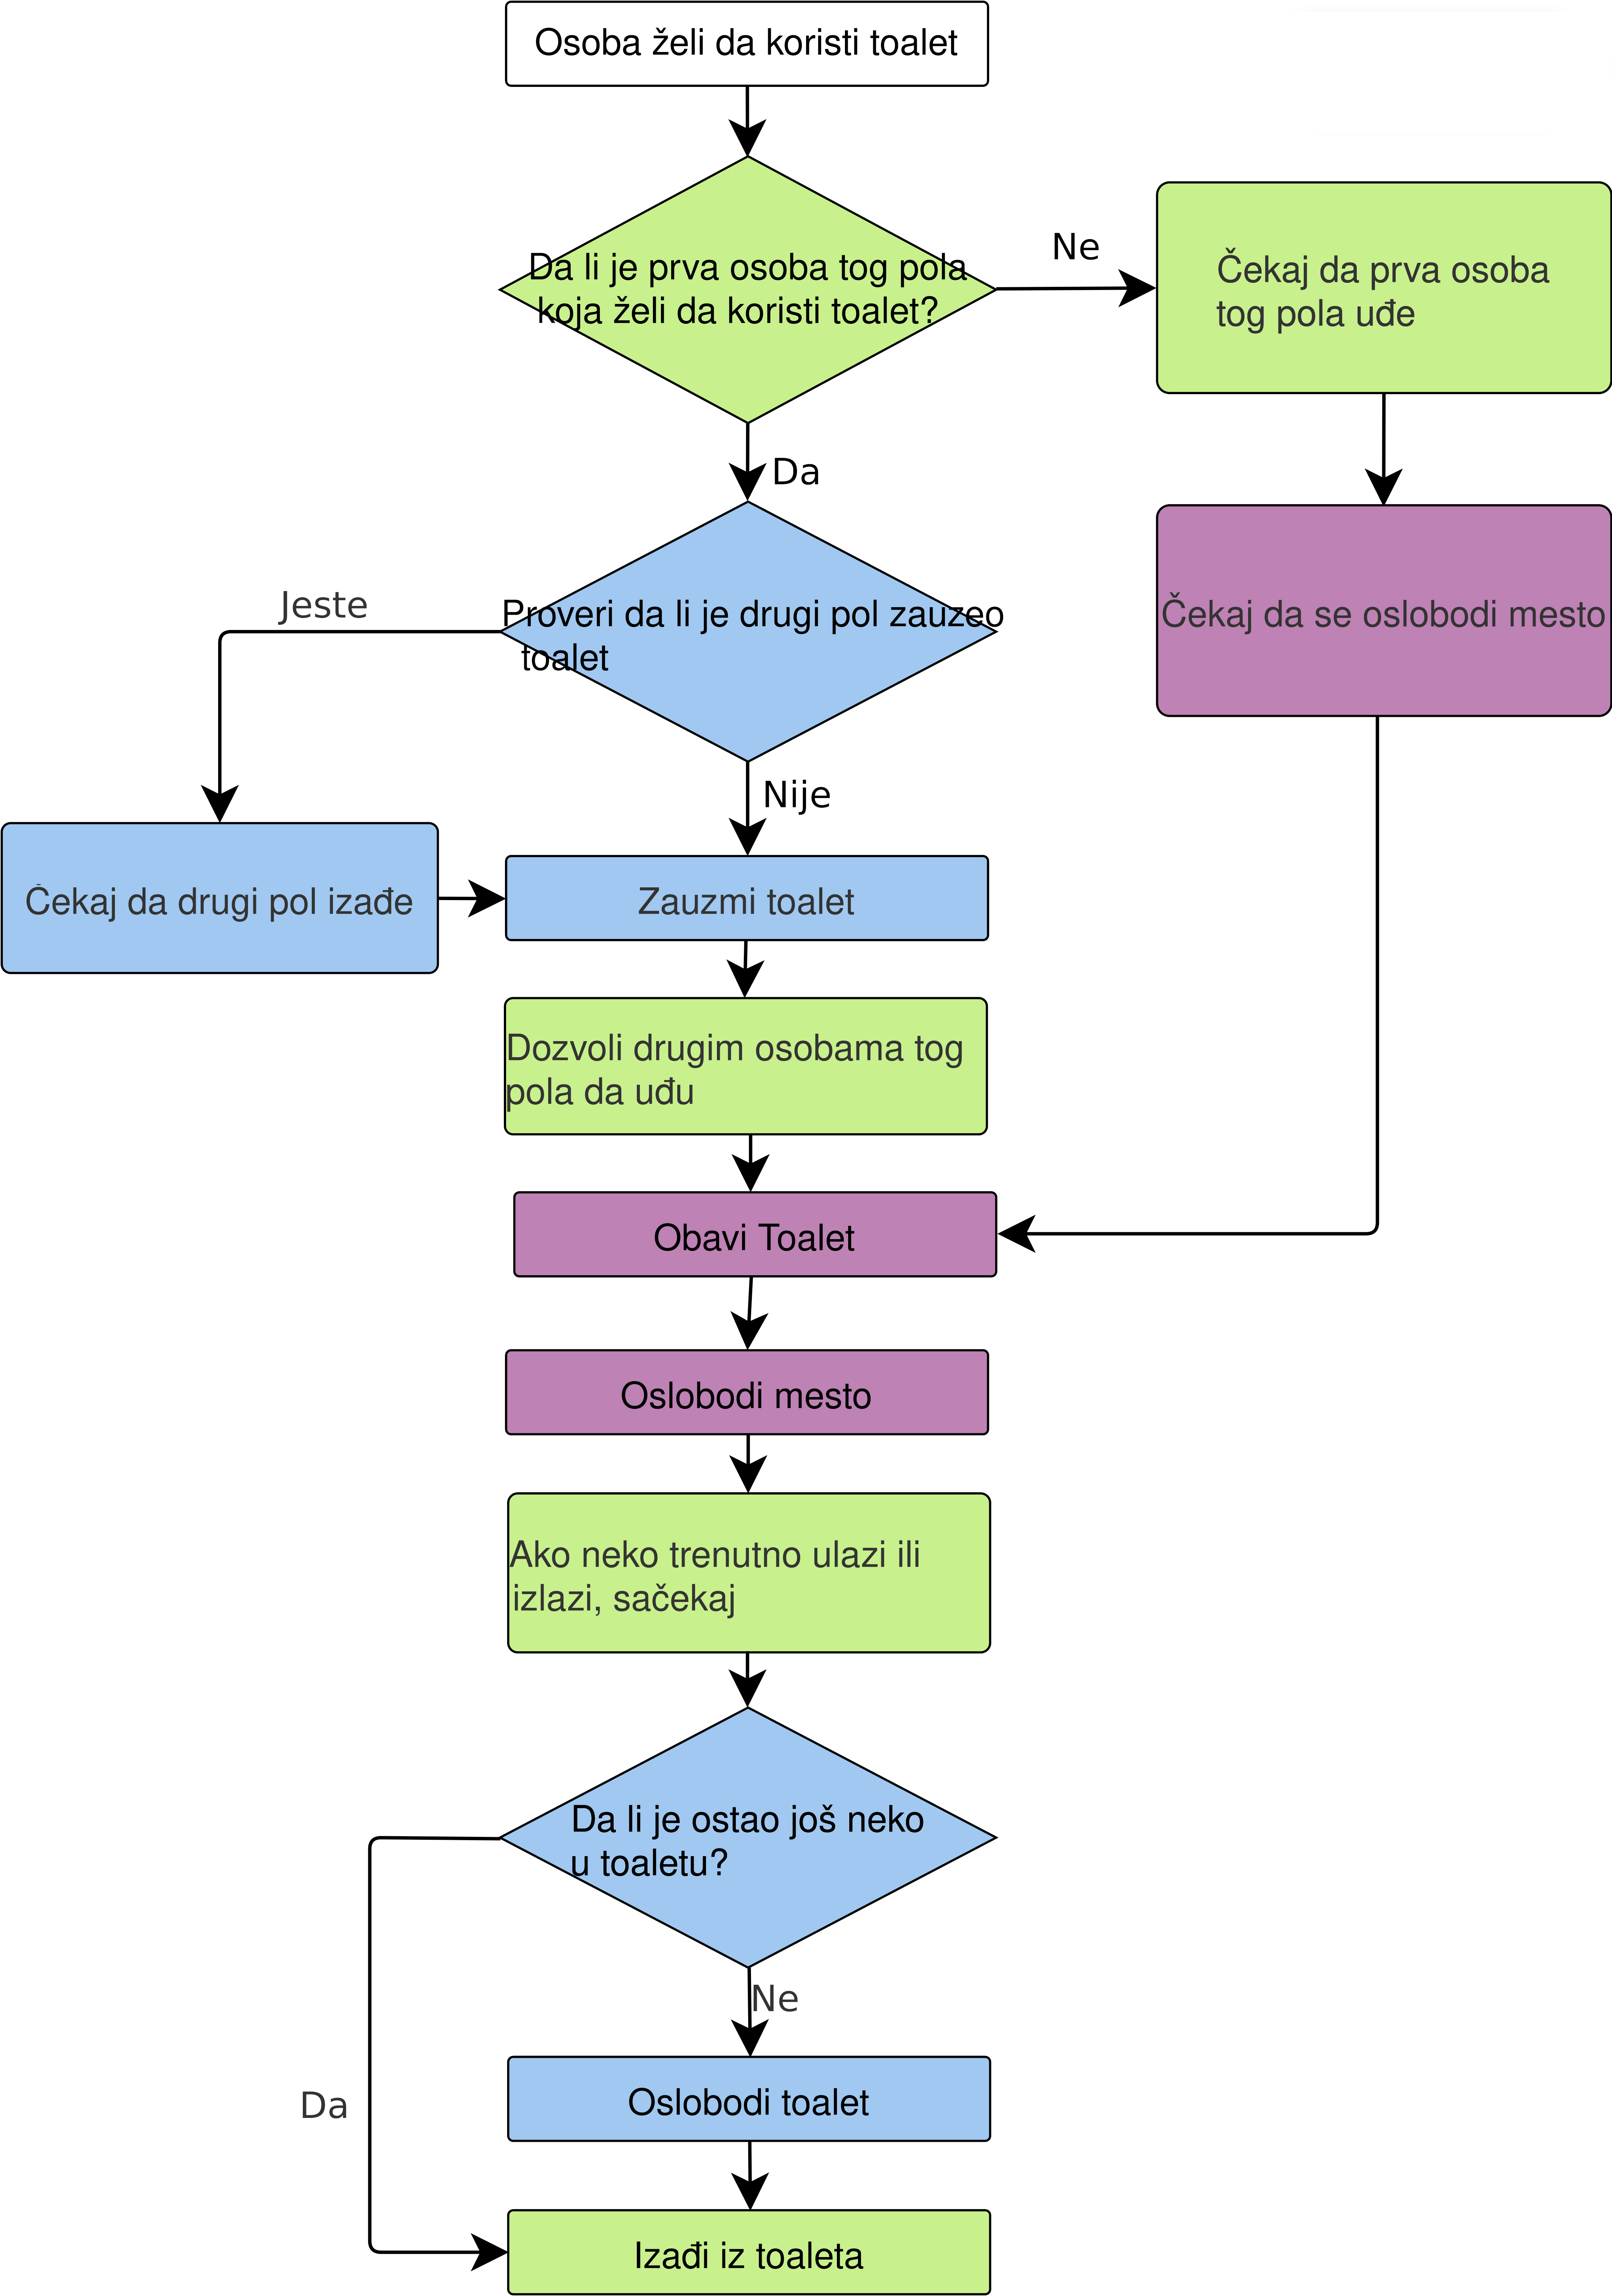
\includegraphics[scale=0.4]{figs/Algoritam-flowchart.png}
	\captionof*{figure}{Slika 1: Šematski prikaz algoritma na koji svaka nit
	nailazi}
	\end{center}
	\newpage
	\section{Implementacija}
	\subsection{Klasa Person}
	Klasa kojom se predstavlja osoba je samo struktura gde se čuvaju pol
	i neki broj koji služi da se u ispisu osobe mogu razlikovati, te jasnije
	pokazati dešavanja.
	Pol je predstavljen enumeracijom sa dva člana jer je to najjednostavnije za
	implementaciju ali i C\# ima metode za pretvaranje u string što je korisno
	za ispis.
	\begin{lstlisting}[language={[Sharp]C}]
enum gender {
	MALE,
	FEMALE
};

internal class Person
{
    public gender gender;
    public int id;

    public Person(gender gender, int id)
    {
        this.gender = gender;
        this.id = id;
    }
}
	\end{lstlisting}
	\subsection{Klasa Toilet}
	U ovoj klasi je implementiran algoritam sa slike 1 i predstavlja srž ovog
	zadatka.
	Polja ove klase su svi semafori korišćeni u rešenju sa tim da je dodat i
	semafor poruke, koji dozvoljava samo jednoj niti da ispisuje na konzolu,
	što obezbeđuje smislen redosled poruka.
	Na primer, ako se desi da je muškarac završio sa toaletom, dok on ispiše
	poruku, može svašta da se desi i ispiše na ekran, kada se njegova poruka
	konačno ispiše, ispadne da program ne radi kako je namenjeno.
	Ovaj semafor ne sprečava pojavu da dok se piše poruka brojno stanje ljudi
	promeni.
	Preostalo polje ove klase su dva brojača, jedan za svaki pol, koji služe
	da se prati kada ulazi prva osoba i kada izlazi poslednja osoba.
	Metoda za ispis je vrlo jednostavna i sve što radi je da pre ispisivanja na
	ekran rezerviše semafor za poruke i čim se to završi ga oslobađa.
	\begin{lstlisting}[language={[Sharp]C}]
	public static SemaphoreSlim toilet = new SemaphoreSlim(1);
	public static SemaphoreSlim[] entryMutex = { new SemaphoreSlim(1), new SemaphoreSlim(1), };
	public static SemaphoreSlim seats = new SemaphoreSlim(Program.TOILET_CAPACITY);
	public static SemaphoreSlim messageMutex = new SemaphoreSlim(1);
	public static int[] cnt = { 0, 0 };

	public static void print(string msg)
{
    messageMutex.Wait();
    Console.WriteLine(msg);
    messageMutex.Release();
}
	\end{lstlisting}

	\newpage
	Algoritam sa slike 1 je implementiran u metodi \textbf{SimulateToilet}
	sa tim da mu se prosleđuje lista osoba i za svaku se stvara nova nit.
	Slika 2 prikazuje isto što i slika 1 ali je uz korake dodato koju metodu
	kog semafora one pozivaju.
	Rutine za svaki pol su identične sa tim da koriste drugačiji semafor za
	proveru mogućnosti ulaska, tako da se samo koristi indeks odgovarajućeg
	semafora.
	\begin{lstlisting}[language={[Sharp]C}]
public static void SimulateToilet(List<Person> people)
{
    var stopwatch = new Stopwatch();
    stopwatch.Start();
    Parallel.ForEach(people, person =>
    {
        entryMutex[(int)person.gender].Wait();
        if (++cnt[(int)person.gender] == 1)
        {
            toilet.Wait();
            print($"{person.gender}S occupied the bathroom");
        }
        entryMutex[(int)person.gender].Release();

        seats.Wait();
        print($"{person.gender} {person.id} started using the toilet, Seats free: {seats.CurrentCount}");
        Thread.Sleep(10000);
        seats.Release();
        print($"{person.gender} {person.id} finished using the toilet, Seats free: {seats.CurrentCount}");

        entryMutex[(int)person.gender].Wait();
        if (--cnt[(int)person.gender] == 0)
        {
            print($"{person.gender}S have left he bathroom");
            toilet.Release();
        }
        entryMutex[(int)person.gender].Release();
    });
    stopwatch.Stop();
    print($"Execution time: {(float)stopwatch.ElapsedMilliseconds / 1000}");
}
	\end{lstlisting}
	\begin{center}
	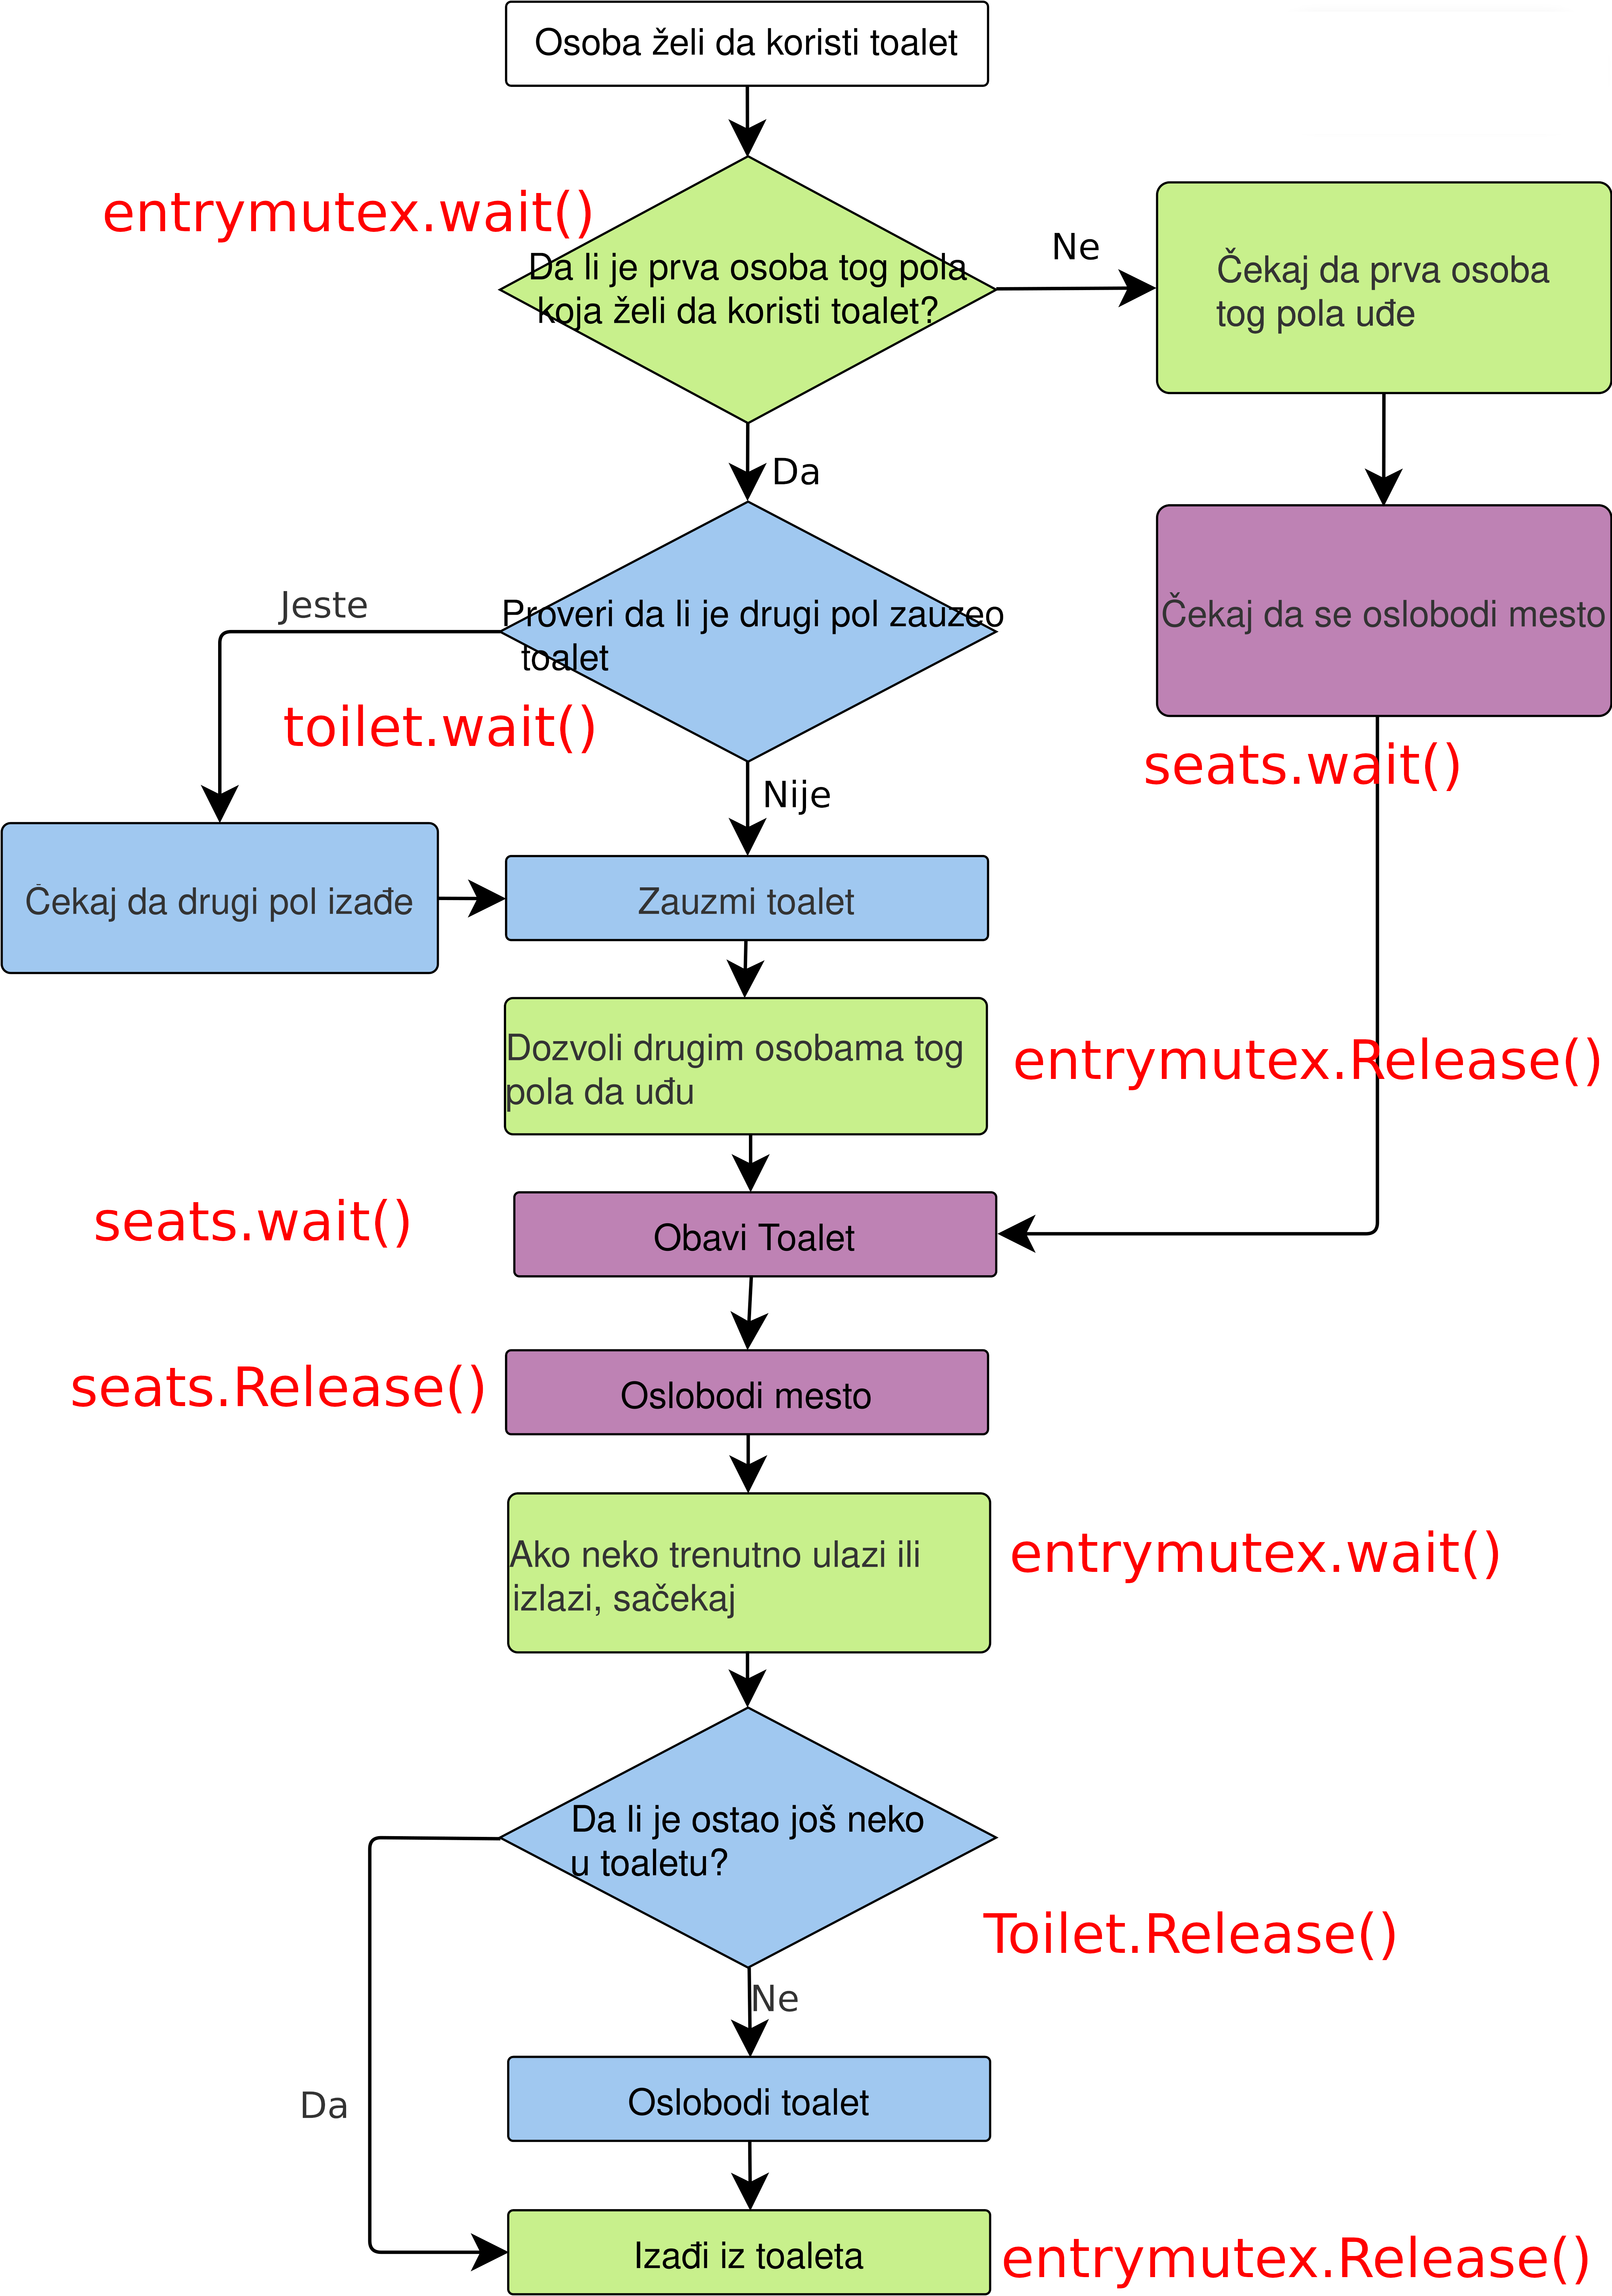
\includegraphics[scale=0.38]{figs/Algoritam-flowchart-funkcije.png}
	\captionof*{figure}{Slika 2: Šematski prikaz algoritma na koji svaka nit
	nailazi sa naznačenim pozivima semafora}
	\end{center}
	\newpage
	\section{Izbegavanje izgladnjivanja}
	Opisano rešenje radi odlično u smislu da žene i muškarci ne mogu istovremeno
	koristiti toalet.
	Međutim problem je to što dok sve osobe jednog pola ne završe toalet,
	drugi pol neće doći na red.
	Mehanizam kojim se to rešava jeste uvođenjem još jednog semafora koji
	propušta do $M$ niti i koji se zauzima čim nit počne da se izvršava, a
	oslobađa pre nego što osoba treba da koristi toalet.
	Jedan apstrakovan način da se o tome razmišlja jeste da ceo red osoba
	koje čekaju ispred toaleta podelimo na dva dela, gde se u jednom delu
	nalazi do $M$ osoba, dok se ostatak nalazi u drugom.
	Tih $M$ osoba su ljudi koji mogu ući u toalet, kako jedna od tih M osoba
	uđe u toalet, osoba iz drugog dela reda prelazi u prvi deo.
	Kada se prvi deo reda napuni osobama pola koje trenutno ne koriste toalet,
	više neće biti osoba koje mogu ući u toalet i kada ga poslednja osoba
	napusti, ljudi iz prvog dela reda počinju da ga koriste tj. menja se koji
	pol trenutno koristi toalet.
	\vspace{0.5cm}
	\begin{lstlisting}[language={[Sharp]C}]
		public static SemaphoreSlim genderSwitch = new SemaphoreSlim(Program.M);
	\end{lstlisting}
	Bitna stvar jeste da što je $M$ manje, pol koji koristi toalet
	će se češće menjati.
	Takođe je važno reći da ako ima više ljudi jednog pola od drugog,
	velika vrednost $M$ dovodi do toga da opet dođe do izgladnjivanja.
	\subsection{Implementacija sa izbegavanjem izgladnjivanja}
	\begin{lstlisting}[language={[Sharp]C}]
public static void SimulateToilet(List<Person> people)
{
    var stopwatch = new Stopwatch();
    stopwatch.Start();
    Parallel.ForEach(people, person =>
    {
        genderSwitch.Wait();
        entryMutex[(int)person.gender].Wait();
        if (++cnt[(int)person.gender] == 1)
        {
            toilet.Wait();
            print($"{person.gender}S occupied the bathroom");
        }
        entryMutex[(int)person.gender].Release();

        genderSwitch.Release();

        seats.Wait();
        print($"{person.gender} {person.id} started using the toilet, Seats free: {seats.CurrentCount}");
        Thread.Sleep(10000);
        seats.Release();
        print($"{person.gender} {person.id} finished using the toilet, Seats free: {seats.CurrentCount}");

        entryMutex[(int)person.gender].Wait();
        if (--cnt[(int)person.gender] == 0)
        {
            print($"{person.gender}S have left he bathroom");
            toilet.Release();
        }
        entryMutex[(int)person.gender].Release();
    });
    stopwatch.Stop();
    print($"Execution time: {(float)stopwatch.ElapsedMilliseconds / 1000}");
}
	\end{lstlisting}
	\newpage
	\section{Rezultat}
	Pre pokretanja programa je potrebno inicijalizovati konstante koje definišu
	kapacitet toaleta, konstantu $M$ tj. podelu reda ljudi koji čekaju da uđu i
	na kraju same ljude.
	U ovom primeru je napravljeno 30 ljudi, i pola su muškarci, a druga polovina
	su žene.
	Ta lista ljudi je prosleđena metodi koja se bavi simulacijom toaleta.
	M je postavljeno kao jedna šestina ukupnog broja ljudi, jer to se pokazalo
	da daje dobru ravnotežu između upotrebe toaleta i učestanosti promene pola
	koji koristi toalet.
	Generalna preporuka je postaviti $M$ da bude trećina broja ljudi od onog pola
	koji je u manjini.
	\begin{lstlisting}[language={[Sharp]C}]
	internal class Program
{
    public const int TOILET_CAPACITY = 4;
    public const int PEOPLE_COUNT = 30;
    public const int M = PEOPLE_COUNT / (2 * 3);

    static void Main(string[] args)
    {
        List<Person> people = new List<Person>();
        for (int i = 0; i < 30; i++)
        {
            if (i < 15) {
                people.Add(new Person(gender.MALE, i));
            } else {
                people.Add(new Person(gender.FEMALE, i));
            }

        }
        Toilet.SimulateToilet(people);
        Console.ReadLine();
    }

}
	\end{lstlisting}
	\par Na slikama 3 i 4 je prikazan rezultat izvršavanja gde je moguće videti
	da se u proseku na svakih 6-7 osoba menja koji pol koristi toalet.
	Takođe se može primetiti da je redosled ispisa poruka dobar ali povremeno
	same poruke prikazuju pogrešan broj slobodnih mesta.
	To se može desiti na više načina, ali glavni način na koji se to ovde dešava
	jeste da izađe jedna osoba, ispiše na ekran broj ostalih mesta tačno, zatim
	druga izađe, ali dok ona ispisuje poruku, druga osoba uđe.
	Jedan način da se to reši jeste da se pristup svim semaforima blokira dok
	se ispisuje poruka, ali to će drastično usporiti program.
	Još jedan način jeste pretvoriti \textbf{print} metodu u makro poziv ili
	\textbf{inline} funkciju, ali to su stvari koje C\# ili ne podržava, ili
	nisu trivijalne za izvesti.
	\begin{center}
	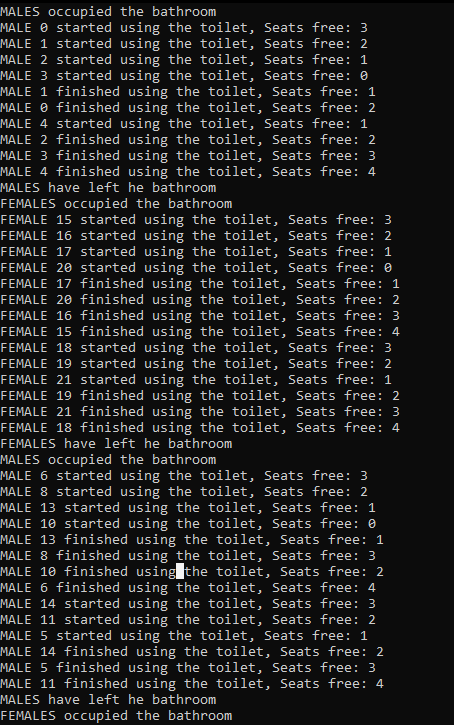
\includegraphics{figs/rezultati1.PNG}
	\captionof*{figure}{Slika 3: Prvi deo prikaza rezultata ivršavanja}
	\end{center}
	\begin{center}
	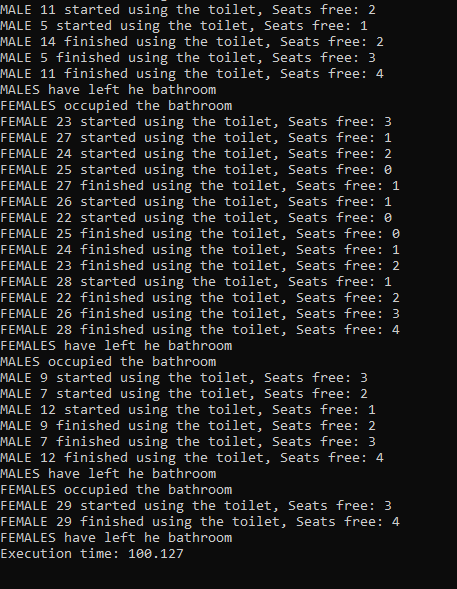
\includegraphics{figs/rezultati2.PNG}
	\captionof*{figure}{Slika 4: Drugi deo prikaza rezultata ivršavanja}
	\end{center}
\end{document}
